حصہ{خطی تخمین اور تفرقات}
بعض اوقات پیچیدہ تفاعل کو سادہ تخمینی تفاعل سے  ظاہر کرتے ہوئے مخصوص موقعوں پر قابل قبول نتائج حاصل کرنا ممکن ہوتا ہے۔ ان سادہ تفاعل کے ساتھ کام کرنا زیادہ آسان ثابت ہوتا ہے۔ اس حصہ میں مماس پر مبنی \اصطلاح{خطی صورتوں}\حاشیہب{linearizations} پر غور کیا گیا ہے۔

ہم نئے متغیرات \عددی{\dif x} اور \عددی{\dif y} متعارف کرتے ہیں جو \عددی{\tfrac{\dif y}{\dif x}} کو نئی معنی دیں گے۔  ہم تجرباتی پیمائش میں خلل اور حساسیت  کو \عددی{\dif y} سے ظاہر کریں گے۔

\جزوحصہء{خطی تخمین}
آپ شکل \حوالہ{شکل_استعمال_منحنی_اور_مماس} میں دیکھ سکتے ہیں کہ منحنی \عددی{y=f(x)} کا مماس نقطہ مماس کے نزدیک منحنی کے قریب رہتا ہے۔نقطہ مماس کے دونوں اطراف چھوٹے وقفہ پر مماس کی \عددی{y} قیمت کو  منحنی کی \عددی{y} تخمینی قیمت تصور کیا جا سکتا ہے۔
\begin{figure}
\centering
\begin{subfigure}{0.5\textwidth}
\centering
\begin{tikzpicture}[font=\small]
\begin{axis}[small,axis lines=middle,xlabel={$x$},ylabel={$y$}]
\addplot[domain=-1:2]{x^2}node[pos=0.9,left]{$y=x^2$};
\addplot[domain=0.2:2]{2*x-1}node[pos=0.7,sloped, below]{$y=2x-1$};
\draw(axis cs:1,1)node[circ]{}node[left]{$(1,1)$};
\end{axis}
\end{tikzpicture}
\caption{منحنی اور اس کا نقطہ $(1,1)$ پر مماس}
\end{subfigure}%
\begin{subfigure}{0.5\textwidth}
\centering
\begin{tikzpicture}[font=\small]
\begin{axis}[small,axis lines=middle,xlabel={$x$},ylabel={$y$}]
\addplot[domain=0.5:1.5]{x^2}node[pos=0.9,left]{$y=x^2$};
\addplot[domain=0.5:1.5]{2*x-1}node[pos=0.7,sloped, below]{$y=2x-1$};
\draw(axis cs:1,1)node[circ]{}node[left]{$(1,1)$};
\end{axis}
\end{tikzpicture}
\caption{نقطہ $(1,1)$ کے نزدیک منحنی اور مماس قریب قریب ہیں}
\end{subfigure}
\begin{subfigure}{0.5\textwidth}
\centering
\begin{tikzpicture}[font=\small]
\begin{axis}[small,axis lines=middle,xlabel={$x$},ylabel={$y$}]
\addplot[domain=0.9:1.11]{x^2}node[pos=0.9,left]{$y=x^2$};
\addplot[domain=0.9:1.11]{2*x-1}node[pos=0.7,sloped, below]{$y=2x-1$};
\draw(axis cs:1,1)node[circ]{}node[left]{$(1,1)$};
\end{axis}
\end{tikzpicture}
\caption{دکھائے گئے وقفہ پر مماس اور منحنی بہت قریب ہیں}
\end{subfigure}%
\begin{subfigure}{0.5\textwidth}
\centering
\begin{tikzpicture}[font=\small]
\begin{axis}[small,axis lines=middle,xlabel={$x$},ylabel={$y$},xtick={0.998,1.002,1},xticklabels={$0.998$,$1.002$,$1$},ytick={0.998,1,1.002},yticklabels={$0.998$,$1$,$1.002$},xmin=0.997]
\addplot[domain=0.998:1.002]{x^2}node[pos=0.9,left]{$y=x^2$};
\addplot[domain=0.998:1.002]{2*x-1}node[pos=0.7,sloped, below]{$y=2x-1$};
\draw(axis cs:1,1)node[circ]{}node[left]{$(1,1)$};
\end{axis}
\end{tikzpicture}
\caption{دکھائے گئے وقفے پر منحنی اور مماس میں فرق کرنا مشکل ہے}
\end{subfigure}
\caption{قابل تفرق منحنی کو نقطہ مماس کے قریب  تخمینی طور پر اس  نقطے کے  مماس سے ظاہر کیا جا سکتا ہے}
\label{شکل_استعمال_منحنی_اور_مماس}
\end{figure}

شکل \حوالہ{شکل_استعمال_منحنی_کا_مماس} کی علامتیت استعمال کرتے ہوئے، نقطہ \عددی{(a,f(a))} سے گزرتے ہوئے مماس کی نقطہ-ڈھلوان مساوات
\begin{align*}
y=f(a)+f'(a)(x-a)
\end{align*}
ہے۔یوں مماس تفاعل
\begin{align*}
L(x)=f(a)+f'(a)(x-a)
\end{align*}
کی ترسیم ہے۔ جب تک یہ خط منحنی کے نزدیک رہے اس کو \عددی{f(x)} کی تخمین تصور کیا جا سکتا ہے۔
\begin{figure}
\centering
\begin{tikzpicture}[font=\small]
\begin{axis}[small,axis lines=middle,xlabel={$x$},ylabel={$y$},xtick={\empty},ytick={\empty},xmin=0,ymin=-0.25]
\addplot[domain=0.5:1.5]{x^2}node[pos=0.9,left]{$y=f(x)$};
\addplot[domain=0.6:1.5]{2*x-1}node[pos=0.7,sloped, below]{$f'(a)$ ڈھلوان};
\draw(axis cs:1,1)node[circ]{}node[left]{$(a,f(a))$};
\draw[dashed](axis cs:1,1)--(axis cs:1,0)node[below]{$a$};
\end{axis}
\end{tikzpicture}
\caption{نقطہ $a$ پر تفاعل $f(x)$ کا مماس $y=f(a)+f'(a)(x-a)$ ہو گا}
\label{شکل_استعمال_منحنی_کا_مماس}
\end{figure}

\ابتدا{تعریف}\\
اگر \عددی{x=a} پر \عددی{f} قابل تفرق ہو تب تخمینی تفاعل
\begin{align}\label{مساوات_استعمال_خطی_تخمین}
L(x)=f(a)+f'(a)(x-a)
\end{align}
نقطہ \عددی{a} پر \عددی{f} کی \اصطلاح{خطی صورت}\فرہنگ{خطی صورت}\حاشیہب{linearization}\فرہنگ{linearization} ہو گی۔  \عددی{f} کی درج ذیل تخمین \عددی{L}
\begin{align*}
f(x)\approx L(x)
\end{align*}
نقطہ \عددی{a} پر تفاعل \عددی{f}کی \اصطلاح{معیاری خطی تخمین}\فرہنگ{خطی!معیاری تخمین}\حاشیہب{standard linear approximation}\فرہنگ{linear!standard approximation} ہے۔ نقطہ \عددی{x=a} اس تخمین کا \اصطلاح{وسط}\فرہنگ{وسط}\حاشیہب{center}\فرہنگ{center} ہے۔
\انتہا{تعریف}
%=========================

\ابتدا{مثال}\شناخت{مثال_استعمال_تخمینی_صورت_الف}
\عددی{x=0} پر \عددی{f(x)=\sqrt{1+x}} کی خطی صورت تلاش کریں۔\\
حل:\quad
ہم \عددی{a=0} پر مساوات \حوالہ{مساوات_استعمال_خطی_تخمین} کی درکار صورت حاصل کرتے ہیں جہاں
\begin{align*}
f'(x)=\frac{1}{2}(1+x)^{-\tfrac{1}{2}}
\end{align*}
لیتے ہوئے \عددی{f(0)=1} اور \عددی{f'(0)=\tfrac{1}{2}} ہوں گے لہٰذا
\begin{align*}
L(x)=f(a)+f'(a)(x-a)=1+\frac{1}{2}(x-0)=1+\frac{x}{2}
\end{align*}
ہو گا۔ شکل \حوالہ{شکل_مثال_استعمال_تخمینی_صورت_الف}-الف میں منحنی اور مماس دکھائے گئے ہیں۔ شکل-ا میں مماسی نقطہ کو ڈبہ میں دکھایا گیا ہے۔اس ڈبے کو شکل-ب میں بڑا کر کے دکھایا گیا ہے۔
\انتہا{مثال}
%==========================
\begin{figure}
\centering
\begin{subfigure}{0.45\textwidth}
\centering
\begin{tikzpicture}[font=\small]
\begin{axis}[clip=false,small,axis lines=middle,xlabel={$x$},ylabel={$y$},xlabel style={at={(current axis.right of origin)},anchor=west},ylabel style={at={(current axis.above origin)},anchor=south},xmin=-1.25]
\addplot[domain=-1:-0.5]{sqrt(1+x)};
\addplot[domain=-0.5:5.2]{sqrt(1+x)}node[pos=0.5,below right]{$y=\sqrt{1+x}$};
\addplot[domain=-1:2]{1+x/2}node[pos=0.75,sloped,above]{$y=1+\tfrac{x}{2}$};
\addplot[domain=1.5:5]{5/4+x/4}node[pos=0.8,sloped,above]{$y=\tfrac{5}{4}+\tfrac{x}{4}$};
\draw(axis cs:0,1)node[circ]{};
\draw(axis cs:3,2)node[circ]{};
\draw(axis cs:-0.2,0.9) rectangle (axis cs:0.2,1.1);
\end{axis}
\end{tikzpicture}
\caption{}
\end{subfigure}\hfill
\begin{subfigure}{0.45\textwidth}
\centering
\begin{tikzpicture}[font=\small]
\begin{axis}[clip=false,small,axis lines=middle,xlabel={$x$},ylabel={$y$},xlabel style={at={(current axis.right of origin)},anchor=west},ylabel style={at={(current axis.above origin)},anchor=south},xmin=-0.11,xmax=0.25,ymin=0.85,ymax=1.15,xtick={-0.1,0.1,0.2},ytick={0.9,1.0,1.1}]
\addplot[domain=-0.1:0.2]{sqrt(1+x)}node[pos=0.8,pin=120:{$y=\sqrt{1+x}$}]{};
\addplot[domain=-0.1:0.2]{1+x/2}node[pos=0.75,pin=-45:{$y=1+\tfrac{x}{2}$}]{};
\end{axis}
\end{tikzpicture}
\caption{}
\end{subfigure}
\caption{نقطہ $x=0$ پر $y=\sqrt{1+x}$ اور اس کا خطی تخمین}
\label{شکل_مثال_استعمال_تخمینی_صورت_الف}
\end{figure}


تخمین \عددی{\sqrt{1+x}\approx 1+\tfrac{x}{2}} (شکل \حوالہ{شکل_مثال_استعمال_تخمینی_صورت_الف}-ب) سے درج ذیل قیمتیں حاصل ہوتی ہیں۔
\begin{align*}
\sqrt{1.2}&\approx 1+\frac{0.2}{2}=1.10&& \text{\RL{$2$ اعشاریہ درست}}\\
\sqrt{1.05}&\approx 1+\frac{0.05}{2}=1.025&& \text{\RL{$3$ اعشاریہ درست}}\\
\sqrt{1.005}&\approx 1+\frac{0.005}{2}=1.00250&& \text{\RL{$5$ اعشاریہ درست}}\\
\end{align*}

وسط سے دور خطی تخمینی میں خلل نا قابل نظر انداز ہو گا۔یوں \عددی{\sqrt{1+x}=1+\tfrac{x}{2}} کو \عددی{x=3} کے نزدیک استعمال نہیں کیا جا سکتا ہے۔ آپ کو \عددی{x=3} پر نیا خطی تخمین حاصل کرنا ہو گا۔

\ابتدا{مثال}
\عددی{x=3} پر تفاعل \عددی{f(x)=\sqrt{1+x}} کا خطی تخمین حاصل کریں۔ \\
حل:\quad
ہم \عددی{a=3} پر مساوات \حوالہ{مساوات_استعمال_خطی_تخمین} کی درکار صورت حاصل کرتے ہیں جہاں
\begin{align*}
f(3)=2,\quad f'(3)=\left.\frac{1}{2}(1+x)^{-\tfrac{1}{2}}\right|_{x=3}=\frac{1}{4}
\end{align*}
ہے لہٰذا
\begin{align*}
L(x)=2+\frac{1}{4}(x-3)=\frac{5}{4}+\frac{x}{4}
\end{align*}
ہو گا (شکل \حوالہ{شکل_مثال_استعمال_تخمینی_صورت_الف}-ا)۔ اس خطی تخمین سے \عددی{x=3.2} پر 
\begin{align*}
\sqrt{1+x}=\sqrt{1+3.2}\approx \frac{5}{4}+\frac{3.2}{4}=1.250+0.800=2.050
\end{align*}
حاصل ہوتا ہے جو بالکل درست جواب \عددی{\sqrt{4.2}\approx 2.04939} سے \عددی{\num{0.00061}} ہٹ کر ہے۔

اگر ہم مثال \حوالہ{مثال_استعمال_تخمینی_صورت_الف} میں حاصل خطی تخمین استعمال کریں تب 
\begin{align*}
\sqrt{+x}=\sqrt{1+3.2}\approx 1+\frac{3.2}{2}=1+1.6=2.6
\end{align*}
حاصل ہو گا جس میں \عددی{\SI{25}{\percent}} خلل پایا جاتا ہے۔
\انتہا{مثال}
%================
\ابتدا{مثال}
جذر اور طاق کے لئے اہم ترین خطی تخمین درج ذیل ہے۔
\begin{align}\label{مساوات_استعمال_طاقت_خطی_تخمین}
(1+x)^k&\approx 1+kx&&\text{\RL{$k$ کوئی عدد ہے؛ $x\approx 0$}}
\end{align}
\عددی{x=0} کے نزدیک یہ قابل قبول نتائج دیتا ہے اور یہ وسیع طور استعمال ہوتا ہے۔
\انتہا{مثال}
%===========================

مساوات \حوالہ{مساوات_استعمال_طاقت_خطی_تخمین} سے درج ذیل کلیات اخذ کیے جا سکتے ہیں جن کا وسط \عددی{x=0} ہے۔
\begin{align*}
\sqrt{1+x}&=(1+x)^{\tfrac{1}{2}}\approx 1+\frac{x}{2}&& k=\frac{1}{2}\\
\frac{1}{1-x}&=(1-x)^{-1}\approx 1+(-1)(-x)=1+x&&k=-1\\
\sqrt[3]{1+5x^4}&=(1+5x^4)^{\tfrac{1}{3}}=1+\frac{1}{3}(5x^4)=1+\frac{5}{3}x^4&&k=\frac{1}{3}\\
\frac{1}{\sqrt{1-x^2}}&=(1-x^2)^{-\tfrac{1}{2}}\approx 1+(-\tfrac{1}{2})(-x^2)=1+\frac{x^2}{2}&&k=-\frac{1}{2}
\end{align*}
دیگر اہم خطی تخمین درج ذیل ہیں (اس حصہ کے آخر میں دیے سوالات میں  آپ انہیں اخذ کریں گے) جن کا وسط \عددی{x=0} ہے۔
\begin{align*}
\sin x&\approx x\\
\cos x&\approx 1\\
\tan x&\approx x
\end{align*}
\ابتدا{مثال}\شناخت{مثال_استعمال_خطی_تخمین_کوسائن}
\عددی{x=\tfrac{\pi}{2}} پر \عددی{f(x)=\cos x} کا خطی تخمین حاصل کریں۔\\
حل:\quad
درج ذیل
\begin{align*}
f(\tfrac{\pi}{2})=\cos(\tfrac{\pi}{2})=0,\quad f'(\tfrac{\pi}{2})=-\sin(\tfrac{\pi}{2})=-1
\end{align*}
لیتے ہوئے خطی تخمین درج ذیل ہو گا (شکل \حوالہ{شکل_مثال_استعمال_خطی_تخمین_کوسائن})۔
\begin{align*}
L(x)=f(a)+f'(a)(x-a)=0+(-1)(x-\tfrac{\pi}{2})=-x+\tfrac{\pi}{2}
\end{align*}
\انتہا{مثال}
%=============================
\begin{figure}
\centering
\begin{tikzpicture}
\pgfmathsetmacro{\a}{3/2*pi}
\pgfmathsetmacro{\b}{pi/2}
\begin{axis}[clip=false,small,axis lines=middle,xlabel={$x$},ylabel={$y$},xlabel style={at={(current axis.right of origin)},anchor=west},ylabel style={at={(current axis.above origin)},anchor=south},ymax=1.5,xmax=5.2,xtick={\b},xticklabels={$\tfrac{\pi}{2}$},ytick={\empty}]
\addplot[domain=-\a/6:\a,smooth]{cos(deg(x))}node[pos=0.75,below right]{$y=\cos x$};
\addplot[domain=0.3:3]{-x+pi/2}node[pos=0.1, above right]{$y=-x+\tfrac{\pi}{2}$};
\end{axis}
\end{tikzpicture}
\caption{کوسائن اور نقطہ $x=\tfrac{\pi}{2}$ پر اس کی خطی تخمین}
\label{شکل_مثال_استعمال_خطی_تخمین_کوسائن}
\end{figure}

\جزوحصہء{تفرقات}

